\documentclass{article}
\usepackage[utf8]{inputenc}
\usepackage{graphicx}
\usepackage{array}
\usepackage{adjustbox}
\usepackage[nottoc]{tocbibind}
\title{Progetto sistemi robotici}
\author{Riccardo Villa}
\date{February 2021}


\graphicspath{ ./media/ }

\begin{document}

\maketitle

\section{Introduction}

Il campo dei robot ad uso domestico sta acquisendo sempre più rilevanza con l'aumentare della richiesta di questi ultimi. Ad oggi esistono diverse soluzioni, ma tutte sono piuttosto limitate a task molto specifici.
Le più grosse compagnie conosciute nel campo dei robot per pulizie ad uso domestico sono iRobot Roomba e Neato. I robot di Roomba sono molto efficienti e riescono a coprire anche aree molto difficili da raggiungere, come gli angoli dei muri; inoltre possiedono una varietà di sensori cinetici che permettono a questi robot di avvertire l'ambiente prossimo che li circonda. Ad ogni modo questi robot si muovono casualmente e non mantengono in memoria una mappa delle zone esplorate e di conseguenza non nemmeno coscienza della propria posizione nell'ambiente, a meno di usare un algoritmo chiamato iAdapt.
\paragraph{}
Di contro Neato utilizza un sensore basato su un laser che ruota a 360 gradi per avvertire ed apprendere l'ambiente circostante utilizzando un algoritmo chiamato SLAM.
\paragraph{}
Entrambe le soluzioni di Neato e Roomba sono state ampiamente trattate in letteratura, e la loro oefficienza è indiscussa, tuttavia il loro costo non è irrisorio. Nel seguito si tratterà un algoritmo basato a sua volta su un altro algoritmo pensato per girare su un robot particolarmente economico rispetto ai competor enunciati in precedenza.

\paragraph{}
L'algoritmo a cui ci si è ispirati utilizza solo pochi sensori molto economici: un bumper posto lungo tutto il perimetro del robot per rilevare gli urti e un cliff-sensor posto sotto alg robot per rilevare eventuali scale. A questi vengono poi aggiunti anche un sensore di prossimità a raggi infrarossi ed un sensore TIDAL.
\paragraph{}
L'algoritmo accennato in precedenza appartiene alla categoria di algoritmi casuali, che quindi non mantengono memoria dell'ambiente esplorato; in questo caso tuttavia si manterrà  memoria dell'ambiente esplorato dopo la prima run effettuata con l'algoritmo casuale. Tale mappa verrà poi utilizzata da una piccola AI basata su un algoritmo genetico per trovare il percorso più efficiente possibile da utilizzare a partire dalla seconda run.

\paragraph{}
Anche se ci sarebbero algoritmi più indicati per esplorare l'ambiente (prendono il noem di algoritmi di Area Covering) si è scelto di utilizzare un algoritmo di questo tipo che permetta non solo di esplorare l'ambiente ma anche di pulirlo, perseguendo quinfi la funzione principale del robot.

\paragraph{}
La soluzione trovata dall'algoritmo genetico funzione solo su ambienti statici; se si rilevano cambiamenti all'ambiente l'esecuzione della soluzione ottenuto con l'algoritmo genetico viene sospesa e si innesca nuovamente la strategia basata sull'algoritmo casuale.
\subsection{Ambiente}
L'ambiente in cui si trova il robot viene gestito da una classe Enviroment, la si occupa di simulare tutti gli aspetti relativi all'interazione del robot con l'ambiente. Implementa un metodo per ogni tipo di sensore, che simula la risposta che avrebbe dato un ambiente reale all'interrogazione da parte del sensore.
\subsubsection{Discretizzazione dell'ambiente}
Una pratica comune nell'implementazione degli algoritmi esatti è quella di discretizzare l'ambiente in cui si muove il robot; qui l'ambiente viene discretizzato in una matrice le cui celle sono della stessa dimensione del diametro del robot. Un ostacolo viene espresso segnando come non libere le celle del robot. Se il robot proverà comunque ad andare su una di queste celle si verificherà una collisione. 
\paragraph{}
Ad ogni modo sebbene l'ambiente subisca una discretizzazione, questa viene fatta solo a fini di gestione dell'ambiente stesso e degli ostacoli, ma il robot rimane comunque libero, soprattutto nel primo algoritmo che verrà trattato, di muoversi in un range di posizioni continuo.
\subsubsection{Gestione delle collisioni}
L'ambiente gestisce le collisioni del robot controllando di volta in volta la posizione corrente del robot. Quando il drone è in una posizione tale che il suo perimetro possa intersecare una cella non libera, allora viene generata una collisione e chiamata una funzione dell'ambiente che gestisca quest'ultima.
\paragraph{}
Per annullare anche l'inerzia presente nel sistema fisico del robot al momento dell'impatto viene invocato un metodo implementato direttamente all'interno dei motori del robot che ne azzera l'inerzia.
\paragraph{}
tale funzione segnala la collisione prendendone nota in un attributo dell'ambiente, utile per la valutazione di certi sensori utilizzati per la rilevazione degli urti; in seguito respinge il robot nella più vicina posizione a quella attuale che non generi una collisione. Sebbene un approccio del genere possa risultare pesante è anche il più semplice e sicuro, nonché quello che meglio simula ciò che avviene in un ambiente reale. Per semplicità non viene simulata la componente elastica degli oggetti, dunque il robot quando raggiunge un ostacolo anche a grande velocità si blocca senza rimbalzare.
\section{Caratteristiche fisiche del robot}
Il robot viene implementato attraverso queste caratteristiche fisiche.
Nella simulazione il loro funzionamento e l'interfacciamento con le componenti hardware, come sensori e motori, viene impacchettato nella classe motion system.
\subsection{Apprendimento dell'ambiente}
Il robot possiede  in memoria una matrice di bit di dimensione fissa, su cui verrà mappato l'ambiente circostante, asserendo con 0 le celle libere e con 1 le celle occupate dello spazio discretizzato. Quando il robot rileva di aver percorso abbastanza spazio da aver cambiato cella dello spazio discretizzato interroga il sensore TIDAL sui suoi immediati dintorni e salva il risultato nella matrice. Per evitare problemi di out of bound il robot parte dalla posizione centrale della matrice.

\subsection{Controllori utilizzati}
IL robot utilizza in cascata un controllore di posizione ed un controllore di velocità, entrambi implementati come controllori proporzionali con saturazione. Il controllore in posizione calcola, a partire dalla posizione attuale del robot e dalla posizione da raggiungere, le velocità lineare ed angolare da ottenere per raggiungere l'obbiettivo. Queste velocità target sono passate ad un primo controllore in velocità, che le distribuisce ai controllori di velocità di ciascun motore in modo da ottenere la velocità angolare e lineare voluta. Infine i controllori di velocità di ciascun motore calcolano la forza necessaria per raggiungere la velocità target e restituiscono il corretto voltaggio da applicare al motore a cui sono associati.
\paragraph{}
In questo progetto si sono utilizzate diverse varianti del controllo in posizione a seconda del task da eseguire.


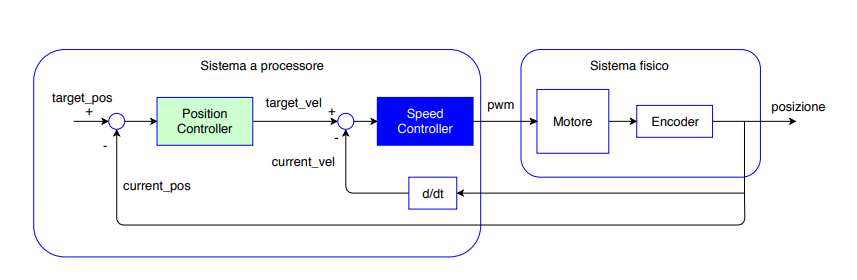
\includegraphics[scale=0.45]{media/schema controllore 1.png}
Il controllore di velocità elabora la velocità lineare e la velocità angolare e stabilisce la velocità target delle singole ruote; valori che vengono passati ai controllori delle singole ruote.
\paragraph{}
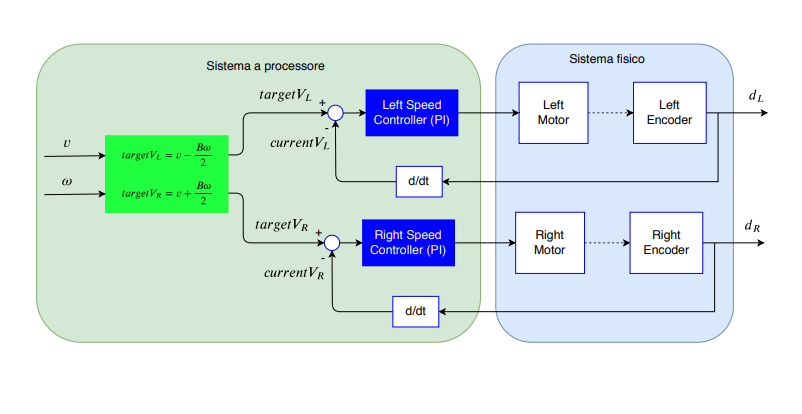
\includegraphics[scale=0.45]{media/schema controllore 2.png}
\subsection{Motori}
Il robot utilizza due motori DC dotati di gearbox associati a ciascuna ruota. I motori dc producono una coppia di forze a partire dalla tensione applicata e dai parametri costruttivi come Resistenza ed impedenza. La velocità di rotazione del motore è ottenuta in funzione della coppia di forze generata e dalla forza resistente. Un riduttore di giri è aggiunto per aumentare la coppia di forze e ridurre il numero di giri del motore.
Il motore è simulato con la classe dc-motor che prende in input l'intensità di corrente, tiene traccia della forza resistente e calcola il numero di giri del motore e la velocità angolare della ruota.

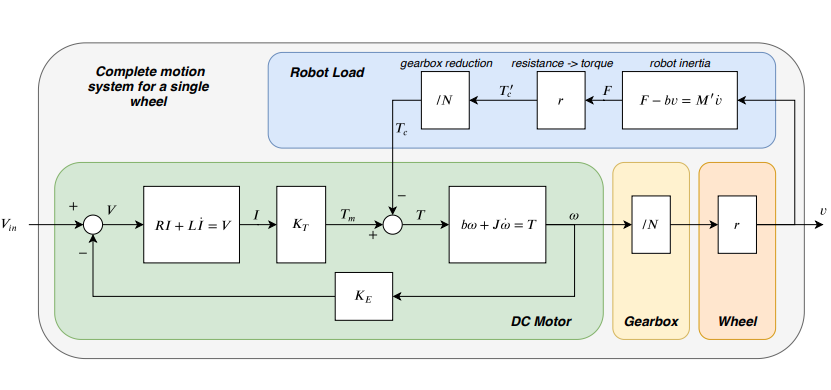
\includegraphics[scale=0.4]{media/schema motore.png}
\subsection{Sensori}
Il robot utilizza una varietà di sensori per diversi scopi.
\subsubsection{Bumper}
Un semplice sensore posto su tutto il perimetro del robot per rilevare urti di una certa intensità. Viene implementato tramite una funzione di environment che viene chiamata quando avviene una collisione ed asserisce un parametro associato al bump, che la chiamata al sensore va a controllare.

\subsubsection{sensore ottico riflessivo}
Questo tipo di sensori si basa sull'emettere un fascio luminoso da fare rimbalzare sull'ostacolo e ritornare al sensore; a seconda della parte di sensore colpita dal raggio di ritorno si calcola l'angolo formato dal raggio e di conseguenza la distanza dall'ostacolo. Solitamente si utilizza un raggio infrarosso dal momento che soffre di meno di eventuali interferenze.\\
Un sensore viene posto davanti al robot e serve a rilevare con precisione la distanza dagli ostacoli verso cui il robot sta andando, in modo che questo possa gradualmente rallentare per non urtarli, ma solo toccarli.
\paragraph{}
L'output fornito dal questo sensore viene direttamente passato in input al controllore in posizione, il quale ritorna una velocità target proporzionale alla distanza dall'ostacolo rilevata dal sensore. Questo permette di avvicinarsi sempre più lentamente ad un' ostacolo fino a raggiungere una distanza tale da considerarlo raggiunto oppure fino a quando il sensore bumper non rileva un urto, che grazie all'azione del d-sensor sarà comunque di lieve entità.

\subsubsection{Tidal sensor}
IL Tidal consiste in un sensore tof che ruota su drone in modo da coprire un raggio d'azione di 360 gradi. Il Time-of-flight, un sensore ad ultrasuoni che fa partire un ultrasuono e rimane in attesa del ritardo con cui ritorna al drone. sulla base di questo si calcola la distanza dall'ostacolo. Viene usato per un compito molto meno delicato rispetto al suo predecessore, cioè rilevare la posizione dell'ostacolo rispetto al drone piuttosto che rilevarne la distanza. Viene usato principalmente per allinearsi ad un' ostacolo dopo che questo è stato rilevato dal d-sensor, dopo che il robot vi si è posto molto vicino.

\subsection{Controlli in posizione}
I controlli sono demandati ad istanze della classe PositionControl, sono delle entità astratte che si pongono un obbiettivo, acquisiscono dati dall'ambiente circostante, elaborano una strategia e si interfacciano con il controllore in velocità per metterla in atto.
\paragraph{}
Gli oggetti di questa classe hanno la possibilità di ricevere un obbiettivo con il metodo set-target(), dopo di che ad ogni chiamata di evaluate acquisiscono dati dal sistema fisico del robot e decidono quali input dare ai controllori. Quando stabiliscono che l'obbiettivo è stato raggiunto il target viene azzerato e le successive chiamate ad evaluate() non sortiranno alcun effetto, fino a ricevere un nuovo obbietti.
\subsubsection{Relative Rotation Control}
Questo controllo si occupa di realizzar una rotazione del robot; con set-target() viene settata l'angolo della rotazione da compiere, e contemporaneamente viene inizializzato un accumulatore associato alla porzione di rotazione attualmente effettuata. A ogni chiamata ad evaluate() il controllo calcola la velocità angolare da raggiungere sulla base della differenza tra la rotazione target e la rotazione già effettuata, e passa questo parametro al controllore in velocità. Non si occupa della velocità lineare, che per default viene posta 0 0.
\subsubsection{Controllo polare}
Prende in input una posizione da raggiungere, e ad ogni evaluate calcola la velocità sia lineare che angolare necessaria per raggiungere tale posizione.
\subsubsection{Dummy control}
Una variante del controllo visto prima. Anziché stabilire a priori un posizione da raggiungere ad ogni chiamata di evaluate() si passa un valore corrispondete alla distanza dall'ostacolo più prossimo lungo la direzione che il robot sta percorrendo al momento.
Il controllo stabilisce la velocità a cui è possibile andare in basa alla distanza dall'ostacolo; questo controllo non si occupa della velocità angolare, che per default viene posta a 0. In pratica questo controllo fa andare il robot dritto fino a fargli toccare delicatamente un ostacolo; a questo punto il target può dirsi raggiunto.
\subsubsection{Allineamento}
Alcuni degli approcci presentati in seguito funzionano meglio se il robot si allinea con i confini dell'ambiente, per poi costeggiarli. Questo viene fatto attraverso il Tidal sensor dopo che il drone si è avvicinato ad un ostacolo; il TIDAl viene usato non per rilevare quanto distante risulti l'ostacolo ma a quale inclinazione del sensore l'ostacolo risulta più vicino, dopo di che il robot ruota finché l'ostacolo non si trova esattamente davanti.

\section{Approccio esplorativo}
L'approccio presentato prevede di alternare 4 diverse strategie di esplorazione casuale per un certo intervallo di tempo nel quale il robot dovrebbe coprire la maggior parte dell'ambiente in cui si trova.

\paragraph{}
Le strategie descritte nel seguito sono realizzate sfruttando altri controllori di più più alto livello:

\subsection{Random Walk}
Il drone cammina in avanti fino a rilevare una collisione con il bump sensor; quando è molto vicino all'ostacolo usa il d-sensor per adeguare la velocità in modo da toccarlo molto piano. In seguito il drone esegue una rotazione casuale in un intervallo di un certo intervallo che eviti di collidere due volte con lo stesso ostacolo.
\begin{center}
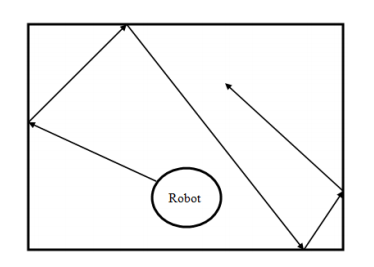
\includegraphics[scale=0.5]{media/random walk.png}
    
\end{center}
\paragraph{}
L'intervallo è determinato a partire dalla posizione dell'ostacolo rispetto al robot. A partire dall'angolo formato tra l'ostacolo e il fronte del robot si esegue una ulteriore rotazione casuale che sommata  a questo angolo risulti nell'intervallo tra 90 e 270.
\subsection{Spirale}
Il robot segue una spirale fino a quando non collide con qualcosa. In questo caso è difficile che l'ostacolo si trovi esattamente davanti al drone, dunque non possiamo fare affidamento sul d-sensor, e dovremo solo usare il Tidal sensor per rallentare ed il bumper per rilevare la collisione.
\begin{center}
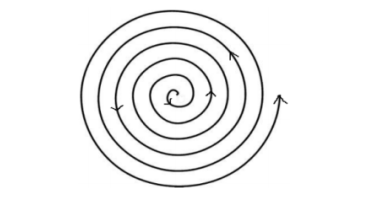
\includegraphics[scale=0.5]{media/spirale.png}
    
\end{center}
\subsubsection{Implementazione}
Per questo approccio si utilizza direttamente il controllore in velocità, passandogli inizialmente una velocità target lineare nulla e una velocità target angolare costante. A questo punto il controllore in velocità fa si che il robot ruoti su se stesso. La velocità lineare viene a poco a poco incrementata in modo che il robot descriva cerchi sempre più ampi, applicando di fatto un moto a spirale.
Ci si ferma quanto si rileva una collisione con il bump sensor, ma si usa il tidal sensor per rilevare a presenza di ostacoli in tutte le direzioni e rallentare di conseguenza, anche se l'ostacolo non era esattamente nella traiettoria del robot.
\begin{center}
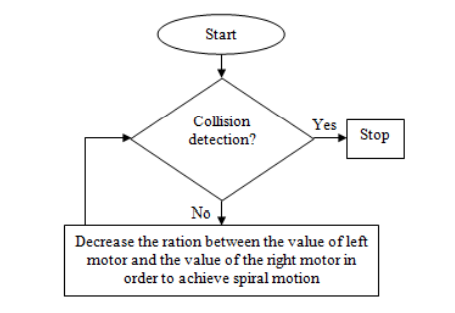
\includegraphics[scale=0.5]{media/schema spirale.png}
    
\end{center}
\subsection{zig-zag}
Il drone segue appunto una strategia a zig-zag; per massimizzare l'efficacia ogni volta che raggiunge un ostacolo si allinea in modo da averlo perfettamente di fronte, e poi compie una rotazione di 90 gradi verso destra o verso sinistra, alternando le due direzioni.
Una volta raggiunta la fine dell'ambiente cambia direzione dello zig zag.
\begin{center}
    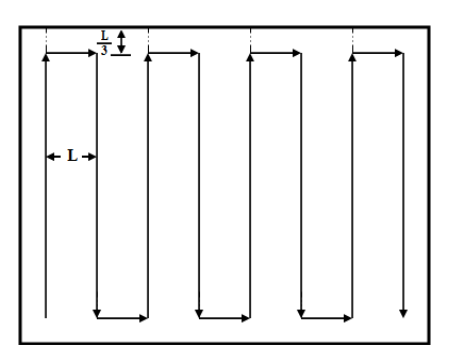
\includegraphics[scale=0.5]{media/zig-zag.png}
\end{center}
\subsubsection{Implementazione}
Questo approccio è implementato attraverso un automa a stati finiti:
\begin{enumerate}
    \item allo stato 0 il drone prosegue fino a raggiungere un ostacolo, raggiunto questo si allinea con quest'ultimo e passa allo stato 2;
    \item lo stato 1 è lo stato in cui il drone prosegue usando il dummy contrl, fino a raggiungere un ostacolo, nel qual caso passa allo stato 2
    \item allo stato 2 viene eseguita una rotazione di 90 gradi, dopo di che si passa allo stato 2.1
    \item allo state 2.1 si prosegue con il dummy control, ma solo per una certa quantità di tempo, dopo di che si passa allo stato 2.2. Se in questo stato si incontrano delle collisioni vuol dire che abbiamo terminato di esplorare lo spazio disponibile con la strategia a zig-zag, e si passa allo stato finale.
    \item allo stato 2.2 si esegue un'altra rotazione di 90 nello stesso verso di quella eseguita allo stato 2, dopo di che si cambia il verso per le future rotazioni e si torna allo stato 1.
\end{enumerate}

\begin{center}
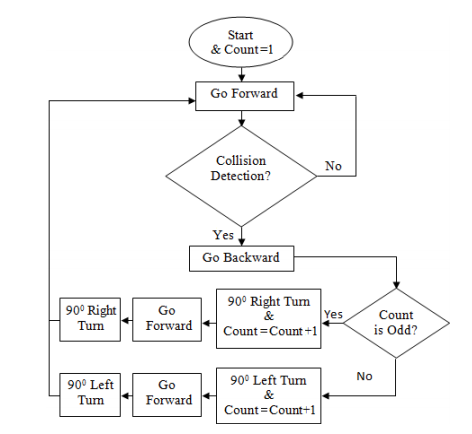
\includegraphics[scale=0.5]{media/sche4ma zig-zag.png}
\end{center}
\subsection{Boundary Walk}
Questa è la strategia che permette di pulire meglio i confini dell'ambiente. consiste appunto nel seguire i confini dell'ambiente rimanendo quanto più possibile allineato a questi.

\begin{center}
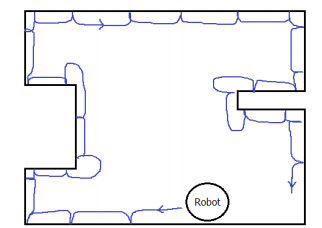
\includegraphics[scale=0.7]{media/boundary walk.png}
\end{center}
\subsubsection{Implementazione}
Appena avviata si prosegue fino ad incontrare un ostacolo e ci si allinea con esso, dopo di che si passa allo stato 1.
\begin{enumerate}
    \item allo stato 1 si prosegue utilizzando il dummy control per una certa quantità di tempo, scaduto il quale o in presenza di una collisione si esegue una rotazione di 90 gradi e si passa allo stato 2. Se si trova un ostacolo sia davanti al drone che dopo la rotazione il drone ruota fino a trovare una direzione libera, in genere quella opposta a quella raggiunta dopo la rotazione, al peggio quella da cui veniva il drone, che quindi ripercorre i suoi passi fino a trovare una direzione libera in cui andare.
    \item in questo stato si prosegue fino ad incontrare un ostacolo, che se il drone ha costeggiato correttamente il muro dovrebbe trovarsi a breve; altrimenti potrebbe accadere che il drone ha superato l'ostacolo che stava costeggiando, e dopo di questo ha trovato un nuovo spazio, in questo caso prosegue fino a trovare un ostacolo in questo nuovo spazio. Una volta trovato l'ostacolo si esegue una breve retromarcia e si esegue una rotazione di 90 gradi nel verso contrario rispetto a quella fatta alla fine dello stato 1; dopo di che si passa nuovamente allo stato 1.
\end{enumerate}

\begin{center}
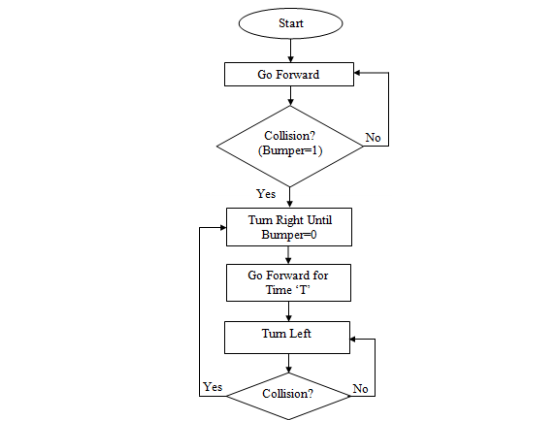
\includegraphics[scale=0.6]{media/schema boundary walk.png}
\end{center}

\subsection{Combinazione degli approcci}
Il controllore così formato prende in input i controllori che implementano 4 approcci visti e pianifica il movimento del robot alternandoli, assegnando a ciascun approccio un tempo di esecuzione scelto dall'utente.


\section{Intelligenza Artificiale}
\subsection{Algoritmo genetico}
L'algoritmo genetico è un algoritmo di tipo euristico basato su popolazione che piuttosto che costruire a poco a poco una soluzione ottima per problemi di difficile soluzione, genera fin dall'inizio una soluzione ammissibile randomica, e tenta di migliorarla per quanto possibile fino ad ottenere una soluzione anche se non ottima quantomeno discreta.
\paragraph{}
L'algoritmo utilizza un popolazione, un insieme di soluzioni ammissibili da migliorare iterazione dopo iterazione con tecniche che verranno esposte nel seguito. Ogni componente della popolazione viene detto individuo o più tecnicamente cromosoma; un cromosoma è formato da un insieme di elementi elementari detti geni.

\subsection{Formalizzazione del problema}
\paragraph{}
Il problema può essere ricondotto ad un problema di ottimizzazione vincolata: vogliamo trovare il numero di mosse di costo minimo sotto il vincolo che il robot visiti tutte le celle libere e nessuna cella occupata da ostacoli, minimizzando il numero di visite effettuate.

\paragraph{}
Questo problema di ottimizzazione può facilmente essere ricondotto ad una istanza del problema del TSP\cite{wiki-TSP} in cui le celle libere sono i vertici del grafo completo in cui vogliamo cercare un ciclo Hamiltoniano.
Il costo di un arco da un vertice ad un suo vertice adiacente è pari ad 1, mentre il costo di un arco da un vertice ad un vertice non adiacente è pari al costo del cammino minimo tra i due vertici.
Nel seguito utilizzeremo l'algoritmo di Dijskra per trovare il cammino minimo tra coppie di vertici, che ben si presta all'ambiente discretizzato, tuttavia in uno scenario reale come quello in cui il robot dovrà muoversi potranno essere usati altri algoritmi di Obstacle Avoidance più indicati (come il dynamic-window-approach\cite{DWA}).
\paragraph{}
Poniamo anche l'attenzione sul fatto che le soluzioni del problema così formalizzato hanno una lunghezza fissa pari al numero di vertici da visitare, non uno di più ne uno di meno; questo rappresenta un grande vantaggio implementativo.
\begin{center}
    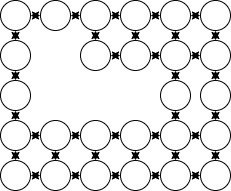
\includegraphics[scale=0.5]{media/graph}
\end{center}
\subsubsection{Complessità del problema}
La soluzione del problema può essere verificata in tempo non polinomiale; quindi il problema presentato appartiene alla classe dei problemi NP. Inoltre come abbiamo visto prima è piuttosto facile ricondurre il problema ad una istanza del TSP, che è noto essere un problema NP-completo, così come anche il suo rilassamento nel piano euclideo eliminando il vincolo di visitare una cella una sola volta. 
\paragraph{}
Dunque abbiamo a che fare con un problema NP-completo; piuttosto che cercare un algoritmo esatto che generi una soluzione ottima presenteremo un approccio euristico per trovare una soluzione approssimata in tempi molto inferiori rispetto a quelli ottenuti da un normale algoritmo esatto.

\section{Risoluzione del problema mediante l'algoritmo Genetico}
In questa sezione di esamina una particolare implementazione dell'algoritmo genetico \cite{10.1007/978-3-642-01970-8_4} e se ne valuteranno eventuali modifiche e prestazioni.
Il problema può essere formalizzato come "trovare la migliore permutazione delle celle libere della matrice", secondo una certa funzione di fitness che vedremo in seguito. Il cromosoma quindi potrebbe essere la sequenza di celle raggiunte dal robot, dove ogni cella raggiunta è un gene; ma per facilitare e rendere più efficaci le operazioni di crossover e mutazioni realizziamo i geni come spostamenti relativi rispetto alla posizione attuale del robot.
\paragraph{}
Il cromosoma
\newcommand{\sep}{\hspace*{.5em}}
  \noindent
  $\fbox{0, 1} \sep \fbox{0, 1} \sep \fbox{0, 1} \sep \fbox{0, 1} \sep \fbox{0, 1}$
porta il robot nella cella $\fbox{0, 5}$.

La posizione $p_i$ raggiunta dal robot al gene $i-esimo$ è definita dall'accumulo degli spostamenti espressi da tutti gli altri geni $p_i = \sum_{j=1}^{i}p_{j}$.
\begin{center}
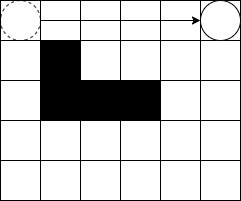
\includegraphics[scale=0.5]{media/image1.png}
\end{center}
\paragraph{}
Uno spostamento in un piano bidimensionale richiede due valori, per asse x e y; per semplificare ulteriormente l'implementazione faremo uso di una funzione che mappa lo spostamento bidimensionale in un unico valore intero positivo, che verrà poi assegnato al gene.
Nel seguito vedremo che questa soluzione offre anche ulteriori vantaggi pratici nelle operazioni di crossover e mutazione, aumentando la variabilità della soluzione anche fra cromosomi tra loro imparentati.

\paragraph{}
Definiamo una funzione $\phi : {\rm I\!R}^2 \rightarrow {\rm I\!N}$ che definisca un certo ordinamento per tutte le possibili mosse che il drone può compiere.
Allora piuttosto che utilizzare direttamente lo spostamento relativo nel gene inseriamo l'indice che questo ha nell'ordinamento definito dalla funzione $p_i = p_{i-1} + \phi(s_i)$ .
Cambiando l'ordinamento assegnato dalla funzione $\phi$ cambia anche la strategia adottata dalla soluzione; quindi potremmo anche assegnare diverse funzioni $\phi$ a diversi cromosomi.
\subsubsection{Esempio}
Per chiarire quanto riportato in precedenza vediamo un esempio di funzioni $\phi$ : nelle tabella in seguito si suppone che il drone si trovi nella casella centrale $[3,3]$; le celle tutt'attorno al drone sono le celle in cui potrebbe andare, in ciascuna cella viene riportato l'indice che lo spostamento necessario al drone per passare dalla cella attuale alla cella designata secondo l'ordinamento definito da una funzione $\phi$.
\begin{center}
\begin{tabular}{ | c | c | c | c | c | c | c | c } 
  \hline
   &  &  & 13 & & & \\
  \hline
   &  &24 &5&14& & \\
  \hline
   & 23 & 12 & 1 & 6 & 15 & \\
  \hline
  22 & 11 & 4 & P1 & 2 & 7 & 16 \\
  \hline
   & 21 & 10 & 3 & 8 & 17 & \\
  \hline
   &  & 20 & 9 & 18 & & \\ 
  \hline
   &  &  & 19 & & & \\  
  \hline
\end{tabular}
\quad
\begin{tabular}{ | c | c | c | c | c | c | c | c } 
  \hline
   &  &  & 19 & & & \\
  \hline
   &  &20 &9&18& & \\
  \hline
   & 21 & 10 & 3 & 8 & 17 & \\
  \hline
  22 & 11 & 4 & P2 & 2 & 7 & 16 \\
  \hline
   & 23 & 12 & 1 & 6 & 15 & \\
  \hline
   &  & 24 & 5 & 14 & & \\ 
  \hline
   &  &  & 13 & & & \\  
  \hline
\end{tabular}
\end{center}
\paragraph{}
Quindi il drone che applica la soluzione che segua l'approccio definito dalla funzione $\phi_1$ controlla se è possibile spostarsi verso l'alto con la mossa [0,1]; se tale cella è libera è non è stata ancora raggiunta ci va, altrimenti controlla se la cella a destra raggiungibile con lo spostamento [1,0] è libera e non è ancora stata raggiunta; se non è possibile controlla la cella in basso, e poi la cella alla sua sinistra. Se nessuna di queste celle è disponibile allora inizia a controllare le celle non adiacenti a quella in cui è posizionato il drone, seguendo l'ordinamento dettato dalla funzione $\phi_1$.

\paragraph{}
Salviamo nei geni l'indice associato alla mossa nell'ordinamento definito dalla funzione associata al cromosoma. Vediamo un esempio di due cromosomi, il primo segue l'approccio definito dalla funzione $\phi_1$, mentre il secondo segue l'approccio definito dalla funzione $\phi_2$.

\paragraph{}
Cromosoma 1:
\begin{center}
\begin{adjustbox}{width=\columnwidth,center}
    \begin{tabular}{ | c | c | c | c | c | c | c | c| c | c | c | c | c | c | c | c| c | c | c | c | c | c | c | c | c | c | } 
  \hline
   2 & 2 & 2 & 2 & 2 & 3 & 3 &3&3&4&1&1&1&4&4&11&3&3&2&2&2&3&4&4&4\\
  \hline
\end{tabular}
\end{adjustbox}
\end{center}

Cromosoma 2:
\begin{center}
\begin{adjustbox}{width=\columnwidth,center}
    \begin{tabular}{ | c | c | c | c | c | c | c | c| c | c | c | c | c | c | c | c| c | c | c | c | c | c | c | c | c | c | } 
  \hline
   1 & 1 & 1 & 1 & 4 & 3 & 4 & 1 & 4 & 3 & 4 & 1 & 4 & 3 & 3 & & 2 & 3 & 2 & 2 & 3 & 2 & 11 & 4 & 4 & 1\\
  \hline
\end{tabular}
\end{adjustbox}
\end{center}

Un altro approccio per risolvere il problema consiste nell'applicare una intelligenza artificiale che produca un cammino esatto per esplorare tutto l'ambiente evitando gli ostacoli nel minor tempo possibile.

Per realizzare l'Intelligenza artificiale è stato utilizzato un algoritmo genetico, che in stanzia una serie di soluzione randomiche dette cromosomi e le migliora iterativamente in maniera più o meno casuale.

Per migliorare le soluzioni vengono usati operatori di crossover, che combinano parti di due soluzioni diverse e mutazioni che cambiano in maniera più o meno randomica parte di una soluzione esplorando lo spazio di ricerca delle soluzioni sperando di trovare una soluzione migliore.

Ad ogni iterazione vengono prodotti nuovi individui, ma solo quelli giudicati i migliori sopravvivono fino all'iterazione successiva avendo modo di riprodursi e creare nuovi individui che ereditino le loro caratteristiche vincenti. A tale scopo viene definita una funzione detta fitness che ha il compito di giudicare la bontà di una soluzione; il valore di output della funzione non è particolarmente importante, purché mantengo l'ordinamento tra le soluzioni.

Facendo evolvere sempre e solo gli individui migliori si rischia di incorrere nel problema dell'overfitting, cioè ci si blocca in un minimo locale dal quale non si riesce ad uscire perché nella popolazione sono rimasti solo individui troppo simili tra loro. Dunque si preferisce dare una possibilità anche agli individui peggiori di evolversi; ovviamente migliore sarà la soluzione maggiori saranno le probabilità che questa possa evolversi nella iterazione successiva.

\subsubsection{Dettagli implementativi}
Per implementare l'ordinamento dato da queste funzioni e possibile mappare ogni spostamento un una tabella hash nella posizione corrispondente all'indice, così facendo il costo di traduzione da un gene alla mossa da effettuare è istantaneo. Tuttavia assegnare a priori un indice ad ogni possibile cella raggiungibile dal robot nell'ambiente, anche piuttosto grande, richiederebbe una quantità di memoria pari anche a 4 volte lo spazio occupato dalla matrice in cui è discretizzato l'ambiente, e questo per ogni possibile ordinamento da implementare. Per tanto si può procedere a calcolare ogni volta lo spostamento proceduralmente scorrendo tutti i possibili spostamenti secondo l'ordine dato fino a trovare quello cercato, oppure si può definire una tabella hash limitata ad una certa quantità di valori; se l'indice contenuto nel gene eccede la dimensione della tabella hash allora si procede ad uno spostamento assoluto sulla cella libera e non ancora visitata più vicina alla posizione attuale. 
\subsection{Popolazione iniziale}
La popolazione iniziale viene generata secondo diverse strategie elementari, sintetizzate da delle funzioni da associate a ciascun cromosoma.
Tali funzioni assegnano una preferenza ad ogni possibile cella nell'ambiente del robot. In generale il robot va nella prima (secondo l'ordinamento definito da funzione del cromosoma) cella libera  e che non sia ancora stata pulita.
Qualora il numero di funzioni a disposizione siano minori rispetto al numero prefissato della popolazione è possibile generare altri cromosomi a partire da quelli già creati dalle sole maschere effettuando dei crossover casuali e delle mutazioni, fino a raggiungere la quota di cromosomi prefissata.

\subsection{Crossover}
Il crossover è l'operazione che prende due cromosomi e li mescola, generando uno o più cromosomi che contengano alcune caratteristiche di ogni genitore. Contestualizzando al problema affrontato l'operazione di crossover tra due cromosomi restituisce un nuovo cromosoma che fino ad un certo punto segue il comportamento di un genitore, e poi segue il comportamento dell'altro.
\paragraph{}
I due genitori non hanno lo stesso ruolo nella generazione del nuovo cromosoma; uno di loro ha una maggiore impronta in quanto trasmette al figlio anche la sua funzione di preferenza.
\paragraph{}
La parte iniziale di lunghezza $i$ random del nuovo figlio viene presa così com'è dal primo genitore (quello che ha fornito la maschera), con la certezza che questa prima parte non incontri alcuna cella occupata.
In seguito si cambia genitore e si prova a seguire il comportamento del secondo genitore. Il punto di incrocio tra i cromosomi può essere controllato tramite una probabilità di crossover $pressure$, che è appunto la probabilità che l'incrocio avvenga ad un  certo gene; maggiore è questa probabilità prima avverrà lo scambio di materiale genetico e dunque il cromosoma risultante avrà meno caratteristiche del genitore 1 e più caratteristiche del genitore 2. Viceversa diminuendo tale probabilità lo scambio avverrà più tardi, e dunque nel cromosoma generato vi sarà più materiale genetico del genitore 1 piuttosto che del genitore 2.
\paragraph{}
Notiamo adesso che la posizione a cui si trova il drone all'$i-esimo$ gene del nuovo cromosoma non è la stessa in cui si troverebbe all'$i-esimo$ gene del secondo cromosoma, ed essendo gli spostamenti relativi alla nuova posizione raggiunta anche tutte le altre posizioni raggiunte seguendo le indicazioni del secondo genitore saranno diverse rispetto a quelle che avrebbe raggiunto il suddetto genitore.
\paragraph{}
Se da una parte questo introduce una maggiore variabilità, ci costringe anche a rinunciare alla consistenza offerta da un cromosoma già formato com'è il secondo genitore. Infatti essendo diverse le celle raggiunte vi è sempre il rischio di ritrovarsi un una cella non libera oppure già pulita generando una collisione. Per tanto ogni gene del secondo genitore va controllato, ed in caso non sia buono si prende la posizione successiva secondo la funzione di priorità del genitore 1.

\paragraph{}
Occorre però fare attenzione a non impostare a valori troppo elevati o troppo bassi questo parametro, altrimenti il cromosoma figlio potrebbe ereditare materiale genetico da un solo genitore, che piuttosto che generare un figlio avrà generato un suo clone. In misura minore questo potrebbe già accadere facendo un crossover tra cromosomi già correlati fra loro, che magari condividono la prima porzione di geni; se il punto di crossover rientrasse in questa prima porzione allora il cromosoma generato sarebbe identico ad uno dei genitori in quanto la porzione di materiale genitori scambiata fra i genitori è identica. Utilizzando una buona euristica per la scelta del miglior partner questo rischio è scongiurato, ma, come vedremo in seguito, è possibile anche operare in fase di selezione della nuova popolazione privilegiando cromosomi unici piuttosto che cromosomi duplicati.

\subsubsection{Altri tipi di crossover}
Oltre alla forma più classica di crossover presentata prima sono state testate anche altre varianti, come la uniform crossover, nella quale lo scambio tra informazioni genetiche dei due geni non avviene una sola volta, ma i genitori continuano ad alternarsi nella generazione del materiale genetico del figlio.

\begin{center}
    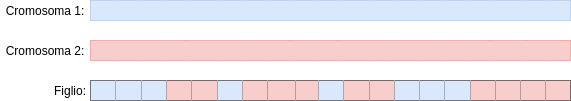
\includegraphics[scale=0.6]{media/unicode.png}
\end{center}

\subsubsection{Implementazione}
Dal punto di vista meramente implementativo possiamo pensare che ricopiamo nel cromosoma generato la prima parte del genitore 1, in seguito andiamo, per ogni gene, ad inserire la prima mossa disponibile secondo la funzione del primo genitore \underline{ma partendo dalla mossa che avrebbe fatto il genitore 2}. 
\paragraph{}
Prima di ricopiare il gene del genitore 2 nel nuovo cromosoma, che ricordiamo usa indici che fanno riferimento alla funzione del genitore 1, questo va "tradotto" per essere usato con la funzione del genitore 1. Il gene del genitore 2 viene tradotto nell'indice che la funzione del genitore 1 associa alla mossa che la funzione del genitore 2 associa alla mossa di indice corrispondente al gene da tradurre.
\paragraph{}
Sia $s_i$ il gene da tradurre e sia $\phi_1(s_i)$ la mossa di indice $s_i$ secondo l'ordinamento definito da $\phi_1$; sia inoltre $\phi_i^T([x,y])$ l'indice assegnato dalla funzione $\phi_i$ alla mossa $[x,y]$ allora la traduzione di un gene $s_{2,i}$ dalla funzione $\phi_2$ alla funzione $\phi_1$ avviene come: $s_{1,i}=\phi_1^T(\phi_2(s_{2_1}))$.

\subsubsection{Esempio di crossover}
Vediamo l'esempio di un crossover tra i cromosomi presentati in precedenza:

\begin{center}
\begin{adjustbox}{width=\columnwidth,center}
   C1: \begin{tabular}{ | c | c | c | c | c | c | c | c| c | c | c | c | c | c | c | c| c | c | c | c | c | c | c | c | c | c | } 
  \hline
   2 & 2 & 2 & 2 & 2 & 3 & 3 &3&3&4&1&1&1&4&4&11&3&3&2&2&2&3&4&4&4\\
  \hline
\end{tabular}
\end{adjustbox}
\end{center}
\begin{center}
\begin{adjustbox}{width=\columnwidth,center}
   C2: \begin{tabular}{ | c | c | c | c | c | c | c | c| c | c | c | c | c | c | c | c| c | c | c | c | c | c | c | c | c | c | } 
  \hline
   1 & 1 & 1 & 1 & 4 & 3 & 4 & 1 & 4 & 3 & 4 & 1 & 4 & 3 & 3 & 2 & 3 & 2 & 2 & 3 & 2 & 11 & 4 & 4 & 1\\
  \hline
\end{tabular}
\end{adjustbox}
\end{center}

Se il nuovo cromosoma eredita la funzione $\phi_1$ del cromosoma 1 allora i geni del cromosoma 2 vanno tradotti prima di essere copiati nel nuovo cromosoma.
\begin{center}
\begin{adjustbox}{width=\columnwidth,center}
   C$2_1$: \begin{tabular}{ | c | c | c | c | c | c | c | c| c | c | c | c | c | c | c | c| c | c | c | c | c | c | c | c | c | c | } 
  \hline
   3 & 3 & 3 & 3 & 2 & 1 & 2 & 3 & 2 & 1 & 2 & 3 & 2 & 1 & 1 & 4 & 1 & 4 & 4 & 1 & 4 & 7 & 2 & 2 & 3 \\
  \hline
\end{tabular}
\end{adjustbox}
\end{center}
Quindi supponendo che lo scambio avvenga nel gene 11 da sinistra il cromosoma risultante sarà:
\begin{center}
\begin{adjustbox}{width=\columnwidth,center}
   C3: \begin{tabular}{ | c | c | c | c | c | c | c | c| c | c | c | c | c | c | c | c| c | c | c | c | c | c | c | c | c | c | } 
  \hline
   2 & 2 & 2 & 2 & 2 & 3 & 3 &3&3&4 & 2 & 3 & 2 & 1 & 1 & 4 & 1 & 4 & 4 & 1 & 4 & 7 & 2 & 2 & 3 \\
  \hline
\end{tabular}
\end{adjustbox}
\end{center}

\subsection{Mutazione}
La mutazione è l'operazione che integra l'esplorabilità delle soluzioni, per uscire da un minimo locale in caso ve ne sia uno.
Come vedremo in seguito l'operazione di mutazione è particolarmente impattante utilizzando gli spostamenti relativi rappresentati come indice di priorità per la funzione.

\paragraph{}
La mutazione prevede di cambiare un singolo gene casuale (controllabile tramite un apposito parametro), assegnandogli un nuovo valore casuale $i$, purché la $i-esima$ migliore mossa della funzione associata al cromosoma sia valida. In caso contrario si assegna al gene mutato la prima migliore mossa possibile successiva alla $i-esima$ mossa secondo l'ordinamento definito dalla funzione $\phi$ assegnata al cromosoma che sta subendo la mutazione.
\paragraph{}
A questo punto la posizione raggiunta al gene i-esimo dopo la mutazione sarà diversa rispetto a quella raggiunta dallo stesso gene prima della mutazione. Questo cambiamento si ripercuote poi su tutto il resto del gene dal momento che usiamo spostamenti relativi; quindi ogni singolo gene dopo i va ricontrollato e per ciascuno va assegnato scelta la prima mossa disponibile secondo la funzione partendo dal valore del gene precedente alla mutazione.
\paragraph{}
Quindi il cromosoma. ottenuto dopo la mutazione potrebbe essere significativamente diverso rispetto al cromosoma prima della mutazione, avendoci così catapultato in un'altra zona dello spazio di ricerca, magari più favorevole.

\subsubsection{soft mutation}
Per non discostarsi troppo da una soluzione già ottima si può tentare di controllare l'impatto della mutazione selezionando il gene da mutare fra i geni che portano ad uno spostamento piccolo, fra celle adiacenti, e mutarlo in un valore che sposti il robot sempre in una cella adiacente a quella del gene mutato.
\paragraph{}
Idealmente se una mutazione normale vorrebbe catapultarci in un altro punto dello spazio di ricerca, la soft mutation vorrebbe piuttosto cercare di esplorare i dintorni della soluzione mutata per cercare un picco migliore. Nell'algoritmo presentato vengono usate sia la mutation che la soft mutation; su una soluzione con un valore di fitness già buono è più probabile che venga usata la soft mutation, invece su una soluzione scarsa è più probabile che venga usata la mutazione classica sperando che porti la soluzione in un punto migliore dello spazio di ricerca.
\paragraph{}
Per selezionare la probabilità di usare la soft mutation si usa il valore di fitness del cromosoma da mutare normalizzato nell'intervallo compreso tra il più alto ed il più basso valore di fitness della popolazione corrente.


\subsubsection{Esempio mutazione}
Vediamo come avviene la mutazione del cromosoma 1 presentato prima. Supponiamo che il gene a subire la mutazione sia il diciannovesimo da sinistra. Il valore del gene 19 viene passato da 2 a 3, e di conseguenza tutti gli alti geni si adattano per non generare collisioni.


\begin{center}
\begin{adjustbox}{width=\columnwidth,center}
   C1: \begin{tabular}{ | c | c | c | c | c | c | c | c| c | c | c | c | c | c | c | c| c | c | c | c | c | c | c | c | c | c | } 
  \hline
   2 & 2 & 2 & 2 & 2 & 3 & 3 &3&3&4&1&1&1&4&4&11&3&3&2&2&2&3&4&4&4\\
  \hline
\end{tabular}
\end{adjustbox}
\end{center}
\begin{center}
\begin{adjustbox}{width=\columnwidth,center}
   $\overline{C1}$: \begin{tabular}{ | c | c | c | c | c | c | c | c| c | c | c | c | c | c | c | c| c | c | c | c | c | c | c | c | c | c | } 
  \hline
   2 & 2 & 2 & 2 & 2 & 3 & 3 & 3 & 3 & 4 & 1 & 1 & 1 & 4 & 4 & 11 & 3 & 3 & \textbf{3} &\textbf 2 &\textbf 1 &\textbf 2 & \textbf2 & \textbf3 & \textbf4\\
  \hline
\end{tabular}
\end{adjustbox}
\end{center}

Aumentando la probabilità della mutazione, il gene mutato sarà più vicino all'inizio del cromosoma, e quindi più geni verranno affetti dalla mutazione, rendendo il gene mutato molto diverso rispetto a quello da cui deriva. Quindi controllando il parametro $p_c$ possiamo anche controllare la potenza della mutazione.

\paragraph{}
Entrambe le operazioni di mutazione, così implementate, presentano un problema: sia $i-esimo$ gene da mutare, se il nuovo valore assegnato al gene dopo la mutazione rappresenta una mossa che precede quella originale nell'ordine definito dalla funzione $\phi$ e se non ci sono mosse possibili prima di quella originale allora la mossa compiuta dal drone sarà sempre quella prima della mutazione; di fatto la mutazione sarà stata nulla.

\subsection{Evoluzione}
\subsubsection{Torneo con elitarismo \cite{Yongsheng} \cite{gfg}}
L'elitarismo consiste nel trasferire nella nuova popolazioni i migliori individui della vecchia popolazione, senza alcuna modifica; la dimensione di questa elité viene stabilita tramite un parametro di elitarismo.
A questo punto però i posti rimasti liberi nella nuova popolazione non sono sufficienti per poter permettere a tutti i cromosomi di potersi evolvere, quindi solo alcuni godranno di questo privilegio, gli altri verranno persi.
\paragraph{}
Per stabilire quali cromosomi debbano evolversi si usa il meccanismo del torneo: un torneo consiste in una sorta di competizione tra i cromosomi partecipanti vinta dal cromosoma con il migliore valore di fitness. Un k-way tournament è un torneo a cui partecipano k individui. Si fanno abbastanza tornei da riempire la nuova popolazione. Il vincitore di ogni torneo viene fatto evolvere.
Per scegliere quali cromosomi debbano partecipare ad ogni torneo si definisce una probabilità $p_t$ di un cromosoma di essere selezionato per gareggiare in un torneo, in questo modo si da una possibilità di evolversi anche a cromosomi con funzione di fitness peggiore dal momento che non è detto che i cromosomi migliori partecipino ad ogni torneo. Questa opportunità può essere ulteriormente sfruttata impedendo ad un individuo che ha già vinto un torneo di partecipare ad altri tornei. 
\paragraph{}
In questo modo abbiamo maggiori possibilità di uscire da eventuali ottimi locali in quanto non facciamo evolvere sempre e soltanto gli stessi cromosomi migliori, ma sfruttiamo anche il materiale genetico di cromosomi che momentaneamente risultano più deboli ma il cui contributo potrebbe essere fondamentale per lasciare situazioni di minimo locale.

\paragraph{}
L'evoluzione consiste dapprima in un crossover con un altro cromosoma, anche non necessariamente fra i candidati ad evolvere, secondo una certa euristica, ed in seguito il cromosoma risultate viene mutato con una certa probabilità $p_m$ per aggiungere delle caratteristiche esplorative all'algoritmo.

\subsection{Implementazione}
L'algoritmo è stato implementato in c; si aspetta di trovare la mappa dell'ambiente in un file input.txt, mentre in output produce un file contenente la migliore soluzione trovata. La soluzione così trovata è salvata su di un file sotto forma di elenco di spostamenti relativi, tra celle adiacenti.

Il file viene quindi letto dal codice del robot e viene generato un elenco di mosse da passare ad un path control() che si occuperà di soddisfare ciascun compito per poi passare a quello successivo.

Per ottimizzare i movimento del robot gli spostamenti simili, cioè lungo la stessa dimensione vengono accorpati in un unico movimento. Per esempio la lita di movimenti [(0,1),(0,1),(0,1),(0,1),(0,1)] che dice al robot di compiere 5 spostamenti verso destra viene accorpata in un unico comando (0,5) che dice al robot di compiere uno spostamento di 5 caselle verso destra.
Ad ogni cambio di direzione viene inserito un comando di rotazione relativa dell'angolo necessario al robot per orientarsi verso la prossima cella da raggiungere relativamente alla direzione attualmente puntata dal robot.



\end{document}
